\documentclass{standalone}
\usepackage{tikz}
\usetikzlibrary{patterns, positioning}
\usepackage[sfdefault]{ClearSans} %% option 'sfdefault' activates Clear Sans as the default text font
\usepackage[T1]{fontenc}

\begin{document}
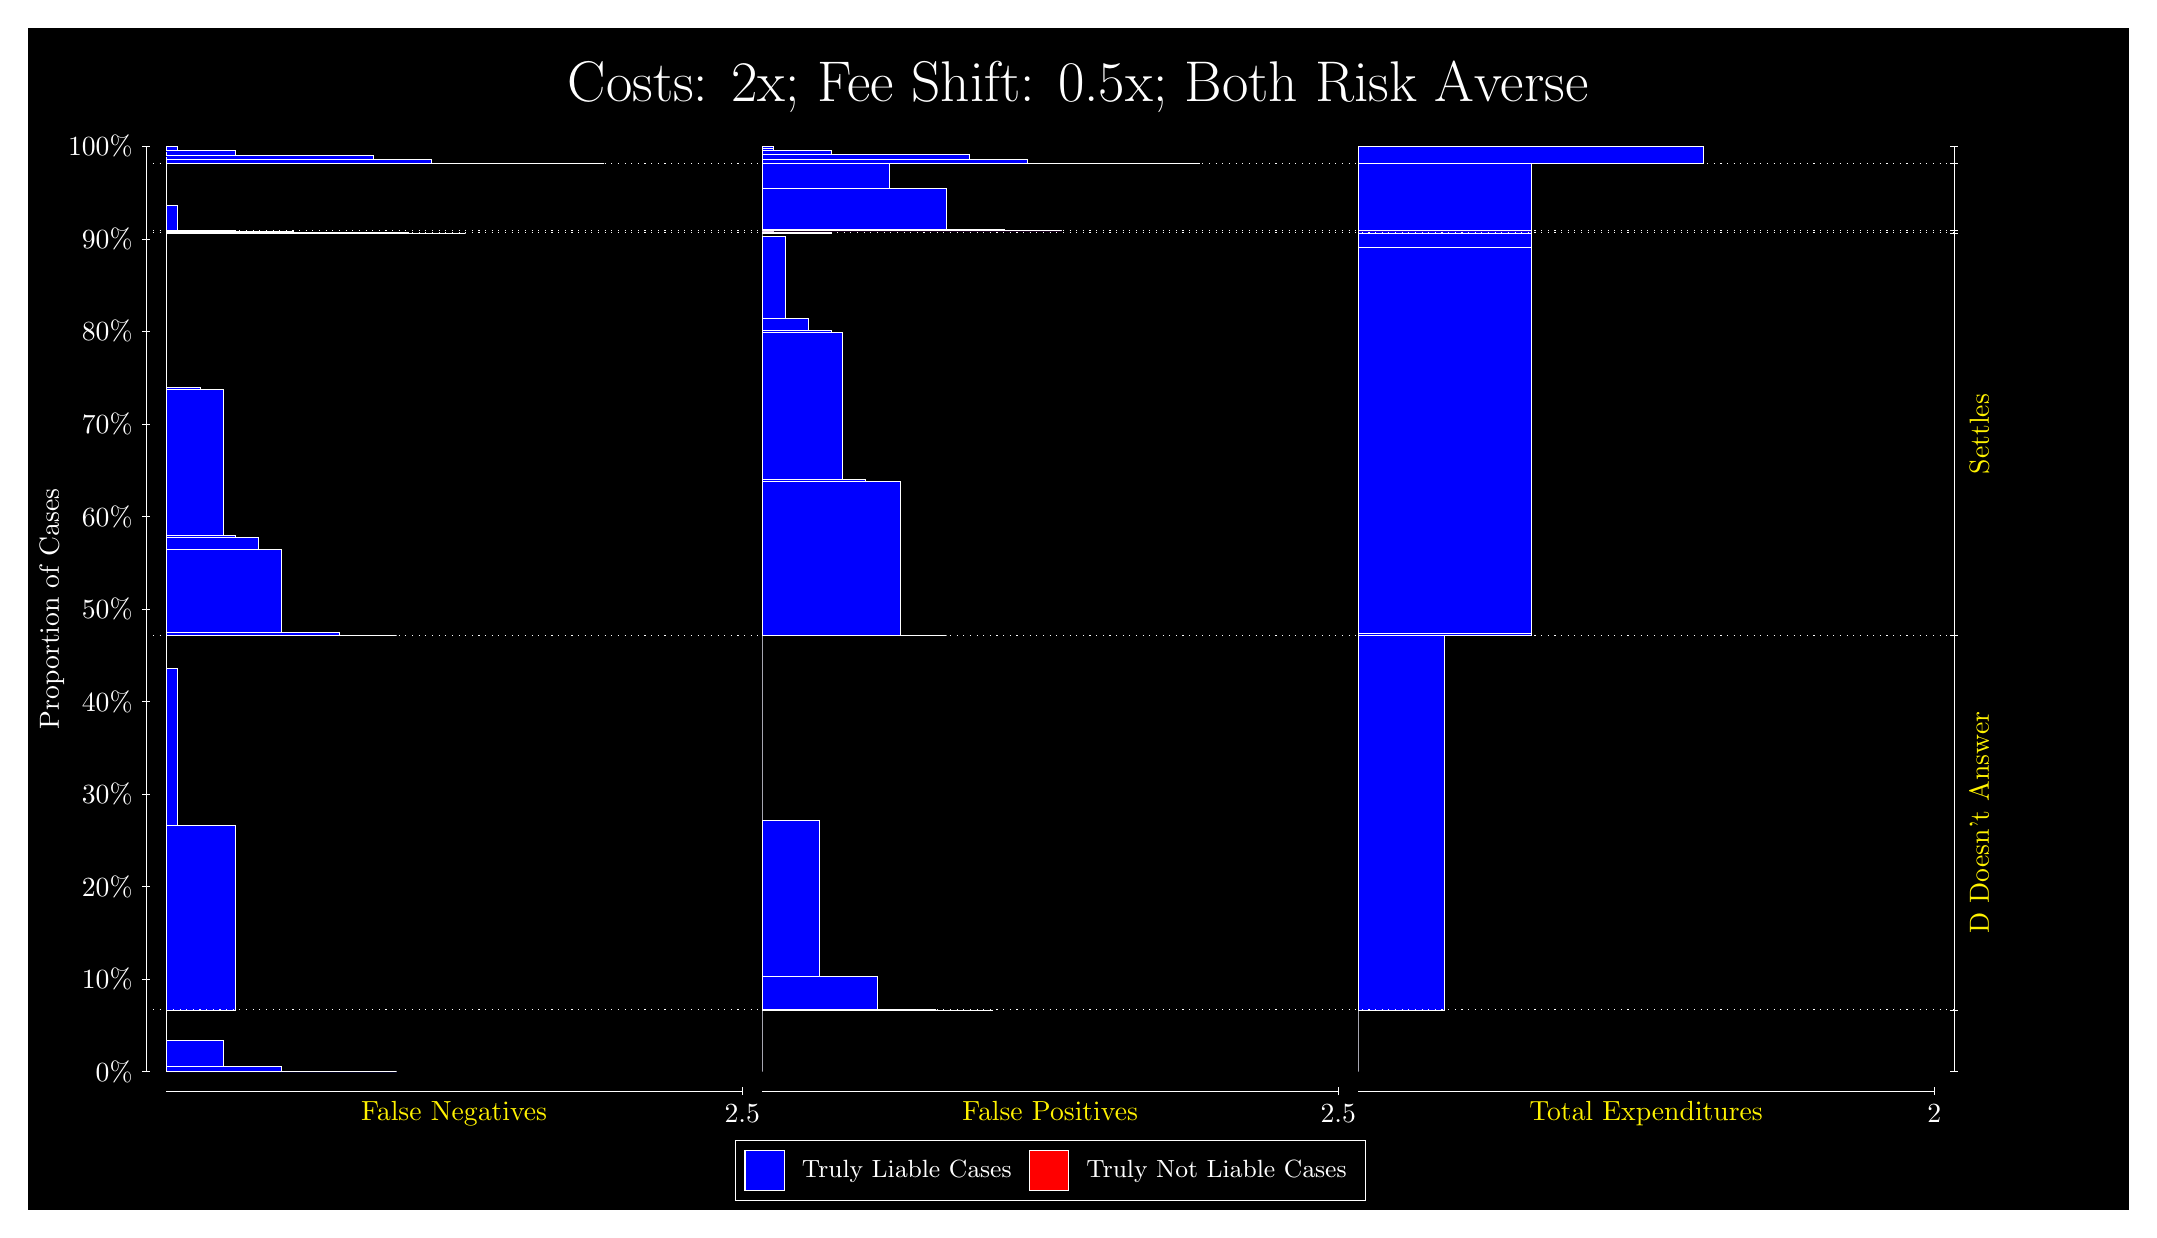
\begin{tikzpicture}
\draw[fill=black] (0,0) rectangle (26.667,15);
\draw[text=white] (0,13.5) rectangle (26.667,15) node[midway] {\huge Costs: 2x; Fee Shift: 0.5x; Both Risk Averse};
\draw[white, very thin] (1.5,1.75) -- (1.5,13.5);
\node[rotate=90, text=white, anchor=center] at (0.3, 7.625) {Proportion of Cases};
\draw[white, very thin] (1.45,1.75) -- (1.55,1.75);
\node[text=white, anchor=east] at (1.45, 1.75) {0\%};
\draw[white, very thin] (1.45,2.925) -- (1.55,2.925);
\node[text=white, anchor=east] at (1.45, 2.925) {10\%};
\draw[white, very thin] (1.45,4.1) -- (1.55,4.1);
\node[text=white, anchor=east] at (1.45, 4.1) {20\%};
\draw[white, very thin] (1.45,5.275) -- (1.55,5.275);
\node[text=white, anchor=east] at (1.45, 5.275) {30\%};
\draw[white, very thin] (1.45,6.45) -- (1.55,6.45);
\node[text=white, anchor=east] at (1.45, 6.45) {40\%};
\draw[white, very thin] (1.45,7.625) -- (1.55,7.625);
\node[text=white, anchor=east] at (1.45, 7.625) {50\%};
\draw[white, very thin] (1.45,8.8) -- (1.55,8.8);
\node[text=white, anchor=east] at (1.45, 8.8) {60\%};
\draw[white, very thin] (1.45,9.975) -- (1.55,9.975);
\node[text=white, anchor=east] at (1.45, 9.975) {70\%};
\draw[white, very thin] (1.45,11.15) -- (1.55,11.15);
\node[text=white, anchor=east] at (1.45, 11.15) {80\%};
\draw[white, very thin] (1.45,12.325) -- (1.55,12.325);
\node[text=white, anchor=east] at (1.45, 12.325) {90\%};
\draw[white, very thin] (1.45,13.5) -- (1.55,13.5);
\node[text=white, anchor=east] at (1.45, 13.5) {100\%};

\draw[white, very thin] (24.457,1.75) -- (24.457,13.5);
\draw[white, very thin] (24.407,1.75) -- (24.507,1.75);
\node[anchor=west] at (24.407, 1.75) {};
\draw[white, very thin] (24.407,2.5332) -- (24.507,2.5332);
\node[anchor=west] at (24.407, 2.5332) {};
\draw[white, very thin] (24.407,7.2881) -- (24.507,7.2881);
\node[anchor=west] at (24.407, 7.2881) {};
\draw[white, very thin] (24.407,12.402) -- (24.507,12.402);
\node[anchor=west] at (24.407, 12.402) {};
\draw[white, very thin] (24.407,12.428) -- (24.507,12.428);
\node[anchor=west] at (24.407, 12.428) {};
\draw[white, very thin] (24.407,13.285) -- (24.507,13.285);
\node[anchor=west] at (24.407, 13.285) {};
\draw[white, very thin] (24.407,13.5) -- (24.507,13.5);
\node[anchor=west] at (24.407, 13.5) {};

\draw[white, very thin, fill=blue] (1.75,1.75) rectangle (4.6775,1.75);
\draw[white, very thin, fill=blue] (1.75,1.75) rectangle (3.9457,1.7505);
\draw[white, very thin, fill=blue] (1.75,1.7505) rectangle (3.2138,1.8127);
\draw[white, very thin, fill=blue] (1.75,1.8127) rectangle (2.4819,2.1421);
\draw[white, very thin, fill=red] (1.75,2.1421) rectangle (1.75,2.1421);
\draw[white, very thin, fill=blue] (1.75,2.1421) rectangle (1.75,2.5332);
\draw[white, very thin, fill=blue] (1.75,2.5332) rectangle (2.6283,4.8794);
\draw[white, very thin, fill=blue] (1.75,4.8794) rectangle (1.8964,6.8662);
\draw[white, very thin, fill=red] (1.75,6.8662) rectangle (1.75,6.8662);
\draw[white, very thin, fill=blue] (1.75,6.8662) rectangle (1.75,7.2881);
\draw[white, very thin, fill=blue] (1.75,7.2881) rectangle (4.6775,7.2881);
\draw[white, very thin, fill=blue] (1.75,7.2881) rectangle (4.3848,7.2881);
\draw[white, very thin, fill=blue] (1.75,7.2881) rectangle (4.092,7.2881);
\draw[white, very thin, fill=blue] (1.75,7.2881) rectangle (3.9457,7.3225);
\draw[white, very thin, fill=blue] (1.75,7.3225) rectangle (3.6529,7.3297);
\draw[white, very thin, fill=blue] (1.75,7.3297) rectangle (3.3602,7.3309);
\draw[white, very thin, fill=blue] (1.75,7.3309) rectangle (3.2138,8.3794);
\draw[white, very thin, fill=blue] (1.75,8.3794) rectangle (2.921,8.5289);
\draw[white, very thin, fill=blue] (1.75,8.5289) rectangle (2.6283,8.554);
\draw[white, very thin, fill=blue] (1.75,8.554) rectangle (2.4819,10.419);
\draw[white, very thin, fill=blue] (1.75,10.419) rectangle (2.1891,10.441);
\draw[white, very thin, fill=blue] (1.75,10.441) rectangle (1.8964,10.445);
\draw[white, very thin, fill=red] (1.75,10.445) rectangle (1.75,10.445);
\draw[white, very thin, fill=blue] (1.75,10.445) rectangle (1.75,12.402);
\draw[white, very thin, fill=blue] (1.75,12.402) rectangle (5.5558,12.402);
\draw[white, very thin, fill=blue] (1.75,12.402) rectangle (4.8239,12.403);
\draw[white, very thin, fill=blue] (1.75,12.403) rectangle (4.092,12.411);
\draw[white, very thin, fill=blue] (1.75,12.411) rectangle (3.3602,12.427);
\draw[white, very thin, fill=blue] (1.75,12.427) rectangle (2.6283,12.428);
\draw[white, very thin, fill=red] (1.75,12.428) rectangle (1.75,12.428);
\draw[white, very thin, fill=blue] (1.75,12.428) rectangle (2.6283,12.431);
\draw[white, very thin, fill=blue] (1.75,12.431) rectangle (1.8964,12.748);
\draw[white, very thin, fill=red] (1.75,12.748) rectangle (1.75,12.748);
\draw[white, very thin, fill=blue] (1.75,12.748) rectangle (1.75,13.285);
\draw[white, very thin, fill=blue] (1.75,13.285) rectangle (7.3123,13.285);
\draw[white, very thin, fill=blue] (1.75,13.285) rectangle (6.5805,13.285);
\draw[white, very thin, fill=blue] (1.75,13.285) rectangle (5.8486,13.288);
\draw[white, very thin, fill=blue] (1.75,13.288) rectangle (5.1167,13.336);
\draw[white, very thin, fill=blue] (1.75,13.336) rectangle (4.8239,13.336);
\draw[white, very thin, fill=blue] (1.75,13.336) rectangle (4.3848,13.381);
\draw[white, very thin, fill=blue] (1.75,13.381) rectangle (4.092,13.381);
\draw[white, very thin, fill=blue] (1.75,13.381) rectangle (3.6529,13.381);
\draw[white, very thin, fill=blue] (1.75,13.381) rectangle (3.3602,13.383);
\draw[white, very thin, fill=blue] (1.75,13.383) rectangle (2.921,13.383);
\draw[white, very thin, fill=blue] (1.75,13.383) rectangle (2.6283,13.383);
\draw[white, very thin, fill=blue] (1.75,13.383) rectangle (2.6283,13.445);
\draw[white, very thin, fill=blue] (1.75,13.445) rectangle (1.8964,13.446);
\draw[white, very thin, fill=blue] (1.75,13.446) rectangle (1.8964,13.495);
\draw[white, very thin, fill=red] (1.75,13.495) rectangle (1.75,13.495);
\draw[white, very thin, fill=blue] (1.75,13.495) rectangle (1.75,13.5);
\draw[white, very thin, fill=red] (9.3189,1.75) rectangle (9.3189,1.75);
\draw[white, very thin, fill=blue] (9.3189,1.75) rectangle (9.3189,2.5332);
\draw[white, very thin, fill=red] (9.3189,2.5332) rectangle (12.246,2.5332);
\draw[white, very thin, fill=blue] (9.3189,2.5332) rectangle (12.246,2.5333);
\draw[white, very thin, fill=blue] (9.3189,2.5333) rectangle (11.515,2.5465);
\draw[white, very thin, fill=blue] (9.3189,2.5465) rectangle (10.783,2.9551);
\draw[white, very thin, fill=blue] (9.3189,2.9551) rectangle (10.051,4.9419);
\draw[white, very thin, fill=blue] (9.3189,4.9419) rectangle (9.3189,7.2881);
\draw[white, very thin, fill=red] (9.3189,7.2881) rectangle (11.661,7.2881);
\draw[white, very thin, fill=blue] (9.3189,7.2881) rectangle (11.661,7.2881);
\draw[white, very thin, fill=red] (9.3189,7.2881) rectangle (11.368,7.2881);
\draw[white, very thin, fill=blue] (9.3189,7.2881) rectangle (11.368,7.2882);
\draw[white, very thin, fill=red] (9.3189,7.2882) rectangle (11.075,7.2882);
\draw[white, very thin, fill=blue] (9.3189,7.2882) rectangle (11.075,9.2455);
\draw[white, very thin, fill=blue] (9.3189,9.2455) rectangle (10.929,9.2492);
\draw[white, very thin, fill=blue] (9.3189,9.2492) rectangle (10.636,9.2716);
\draw[white, very thin, fill=blue] (9.3189,9.2716) rectangle (10.344,11.137);
\draw[white, very thin, fill=blue] (9.3189,11.137) rectangle (10.197,11.162);
\draw[white, very thin, fill=blue] (9.3189,11.162) rectangle (9.9044,11.311);
\draw[white, very thin, fill=blue] (9.3189,11.311) rectangle (9.6116,12.36);
\draw[white, very thin, fill=blue] (9.3189,12.36) rectangle (9.4652,12.361);
\draw[white, very thin, fill=blue] (9.3189,12.361) rectangle (9.3189,12.402);
\draw[white, very thin, fill=red] (9.3189,12.402) rectangle (10.197,12.402);
\draw[white, very thin, fill=blue] (9.3189,12.402) rectangle (10.197,12.403);
\draw[white, very thin, fill=blue] (9.3189,12.403) rectangle (9.4652,12.419);
\draw[white, very thin, fill=blue] (9.3189,12.419) rectangle (9.3189,12.428);
\draw[white, very thin, fill=red] (9.3189,12.428) rectangle (13.125,12.428);
\draw[white, very thin, fill=blue] (9.3189,12.428) rectangle (13.125,12.428);
\draw[white, very thin, fill=blue] (9.3189,12.428) rectangle (12.393,12.443);
\draw[white, very thin, fill=blue] (9.3189,12.443) rectangle (11.661,12.964);
\draw[white, very thin, fill=blue] (9.3189,12.964) rectangle (10.929,13.281);
\draw[white, very thin, fill=blue] (9.3189,13.281) rectangle (10.197,13.285);
\draw[white, very thin, fill=red] (9.3189,13.285) rectangle (14.881,13.285);
\draw[white, very thin, fill=blue] (9.3189,13.285) rectangle (14.881,13.285);
\draw[white, very thin, fill=red] (9.3189,13.285) rectangle (14.149,13.285);
\draw[white, very thin, fill=blue] (9.3189,13.285) rectangle (14.149,13.285);
\draw[white, very thin, fill=red] (9.3189,13.285) rectangle (13.417,13.285);
\draw[white, very thin, fill=blue] (9.3189,13.285) rectangle (13.417,13.29);
\draw[white, very thin, fill=red] (9.3189,13.29) rectangle (12.686,13.29);
\draw[white, very thin, fill=blue] (9.3189,13.29) rectangle (12.686,13.339);
\draw[white, very thin, fill=blue] (9.3189,13.339) rectangle (11.954,13.402);
\draw[white, very thin, fill=red] (9.3189,13.402) rectangle (11.661,13.402);
\draw[white, very thin, fill=blue] (9.3189,13.402) rectangle (11.661,13.402);
\draw[white, very thin, fill=blue] (9.3189,13.402) rectangle (11.222,13.403);
\draw[white, very thin, fill=red] (9.3189,13.403) rectangle (10.929,13.403);
\draw[white, very thin, fill=blue] (9.3189,13.403) rectangle (10.929,13.404);
\draw[white, very thin, fill=blue] (9.3189,13.404) rectangle (10.49,13.404);
\draw[white, very thin, fill=blue] (9.3189,13.404) rectangle (10.197,13.448);
\draw[white, very thin, fill=red] (9.3189,13.448) rectangle (10.197,13.448);
\draw[white, very thin, fill=blue] (9.3189,13.448) rectangle (10.197,13.449);
\draw[white, very thin, fill=blue] (9.3189,13.449) rectangle (9.758,13.449);
\draw[white, very thin, fill=blue] (9.3189,13.449) rectangle (9.4652,13.477);
\draw[white, very thin, fill=blue] (9.3189,13.477) rectangle (9.4652,13.497);
\draw[white, very thin, fill=blue] (9.3189,13.497) rectangle (9.3189,13.5);
\draw[white, very thin, fill=red] (16.888,1.75) rectangle (16.888,1.75);
\draw[white, very thin, fill=blue] (16.888,1.75) rectangle (16.888,2.5332);
\draw[white, very thin, fill=red] (16.888,2.5332) rectangle (17.986,2.5332);
\draw[white, very thin, fill=blue] (16.888,2.5332) rectangle (17.986,7.2881);
\draw[white, very thin, fill=red] (16.888,7.2881) rectangle (19.083,7.2881);
\draw[white, very thin, fill=blue] (16.888,7.2881) rectangle (19.083,7.3182);
\draw[white, very thin, fill=red] (16.888,7.3182) rectangle (19.083,7.3182);
\draw[white, very thin, fill=blue] (16.888,7.3182) rectangle (19.083,12.223);
\draw[white, very thin, fill=red] (16.888,12.223) rectangle (19.083,12.223);
\draw[white, very thin, fill=blue] (16.888,12.223) rectangle (19.083,12.402);
\draw[white, very thin, fill=red] (16.888,12.402) rectangle (19.083,12.402);
\draw[white, very thin, fill=blue] (16.888,12.402) rectangle (19.083,12.428);
\draw[white, very thin, fill=red] (16.888,12.428) rectangle (19.083,12.428);
\draw[white, very thin, fill=blue] (16.888,12.428) rectangle (19.083,13.285);
\draw[white, very thin, fill=red] (16.888,13.285) rectangle (21.279,13.285);
\draw[white, very thin, fill=blue] (16.888,13.285) rectangle (21.279,13.5);
\draw[white, dotted] (1.5,2.5332) -- (24.457,2.5332);
\draw[white, dotted] (1.5,7.2881) -- (24.457,7.2881);
\draw[white, dotted] (1.5,12.402) -- (24.457,12.402);
\draw[white, dotted] (1.5,12.428) -- (24.457,12.428);
\draw[white, dotted] (1.5,13.285) -- (24.457,13.285);
\draw[white, very thin] (1.75,1.5) -- (9.0689,1.5);
\node[text=yellow, anchor=north] at (5.4094, 1.5) {False Negatives};
\draw[white, very thin] (9.0689,1.45) -- (9.0689,1.55);
\node[text=white, anchor=north] at (9.0689, 1.45) {2.5};

\draw[white, very thin] (9.3189,1.5) -- (16.638,1.5);
\node[text=yellow, anchor=north] at (12.978, 1.5) {False Positives};
\draw[white, very thin] (16.638,1.45) -- (16.638,1.55);
\node[text=white, anchor=north] at (16.638, 1.45) {2.5};

\draw[white, very thin] (16.888,1.5) -- (24.207,1.5);
\node[text=yellow, anchor=north] at (20.547, 1.5) {Total Expenditures};
\draw[white, very thin] (24.207,1.45) -- (24.207,1.55);
\node[text=white, anchor=north] at (24.207, 1.45) {2};


\node[text=yellow, centered, rotate=90] at (24.777, 4.9106) {D Doesn't Answer};
\node[text=yellow, centered, rotate=90] at (24.777, 9.8453) {Settles};




\draw (12.978300999999998,1.5) node[draw=none] (baseCoordinate) {};
\begin{scope}[align=center]
        \matrix[scale=0.5, draw=white, below=0.5cm of baseCoordinate, nodes={draw}, column sep=0.1cm]{
            \node[rectangle, draw, minimum width=0.5cm, minimum height=0.5cm, fill=blue] {}; &
            \node[draw=none, font=\small, text=white] (B) {Truly Liable Cases}; &
            \node[rectangle, draw, minimum width=0.5cm, minimum height=0.5cm, fill=red] {}; &
            \node[draw=none, font=\small, text=white] (B) {Truly Not Liable Cases}; \\
            };
\end{scope}

\end{tikzpicture}
\end{document}